\chapter{Intrabundle - An OSGi Bundle Introspection Tool}


\section{Introduction}
With was clear in previous chapters that modular and non modular applications have many differences and specific features hence the need for dedicated approach for quality analysis. This chapter presents a tool called \emph{Intrabundle}\citep{intrabundle github 2014}, an open source Java based application created in the context of this work. Intrabundle introspects OSGi projects collecting useful information and calculates OSGi bundle and project \textbf{internal quality}.  


\section{Design Decisions}
To analyze and extract data from large code bases of OSGi projects which can vary from KLOCs to thousands of KLOCs we needed a lightweight approach with the following non functional requirements:

\begin{itemize}
\item Only open sourced projects because we focus on internal quality where the code is important;
\item The tool should be lightweight to analyze real, complex and huge OSGi projects;
\item 
\item Use Java to leverage the author's experience in the language.
\end{itemize}

Some functional requirements were:

\begin{itemize}
\item Analyze different formats of OSGi projects like Maven\footnote{\href{http://maven.apache.org/index.html}{Maven} is a build tool for Java}, 
Eclipse projects and BND\footnote{\href{http://bndtools.org/}{BND} is a tool to easy OSGi projects development}; 
\item Find and Introspect manifest files
\item It should be able to dive deep into projects source code like counting methods calls, differentiate classes and interfaces and so on;  
\item Get general informations like project version, revision or latest commit in source repository
\item 
\end{itemize}

The following alternatives were evaluated:



\section{Implementation Overview}
identify OSGI project/bundle
extract information
feed metrics
calculate quality

\section{Identifying OSGi Projects and Bundles}

\section{Collecting Bundle Data}

\section{Metrics Calculation}
The data collected earlier will be materialized into six metrics that will be used to calculate OSGi projects quality  

\section{Intrabundle Quality}
In this section we will see how Intrabundle's quality is managed and how some concepts of \textit{section \ref{sec:quality}} were applied to the project. As the project is not OSGi based we can't apply Intrabundle's metrics on itself so we used classical approaches to assure the quality of the project.

\subsection{Internal quality}
Intrabundle internal is managed by PMD and JaCoCo. PMD is an static analysis tool and JaCoCo a dynamic analysis one. Both were presented at Chapter two in section \textit{Quality Analysis Tools} with the objective to guarantee non functional requirements.

\subsubsection{Example}
 PMD was already illustrated at Chapter 2 as an example of static analysis tool. JaCoCo is used to calculate code coverage to track files and methods that automated tests are covering. Figure 3.1 shows JaCoCo code coverage report for Intrabundle:

\begin{figure}[h]
\caption{Intrabundle code coverage}
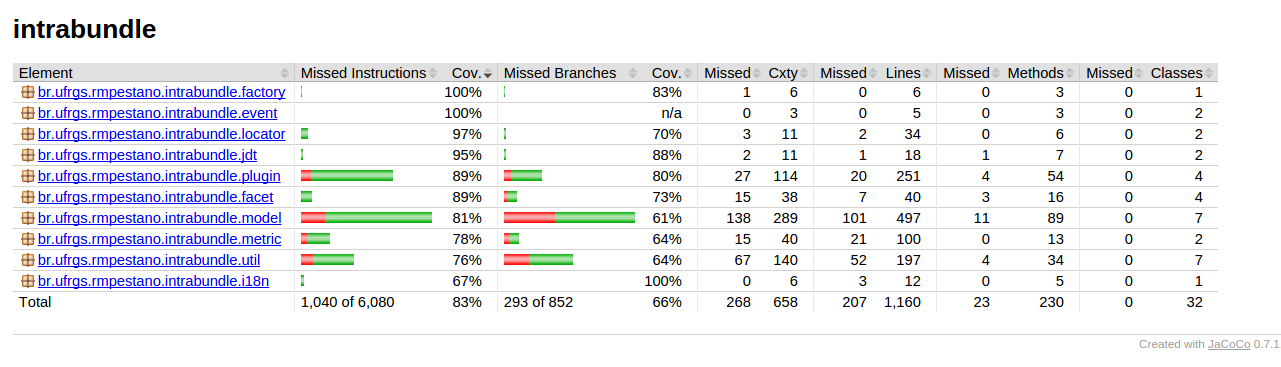
\includegraphics[scale=0.5]{intrabundle-code-coverage}
\end{figure}

\FloatBarrier

\subsection{External quality}
Intrabunde external quality is assured by automated whitebox tests so we can verify if Intrabundle is working as expected, if it meets its functional requirements.

\subsubsection{Example}
As of November 2014 Intrabundle performs 62 \textbf{integration tests} which can be defined as automated tests aimed to detect any inconsistencies between the software units that are integrated together. In this kind of automated tests the system must be running and in case of Intrabundle we also need the Forge runtime up and running during tests and that is done by Arquillian \citep{dan 2011}, an integration test platform. Figure 3.2 shows the result of integration tests execution:

\begin{figure}[h]
\caption{Intrabundle external tests}
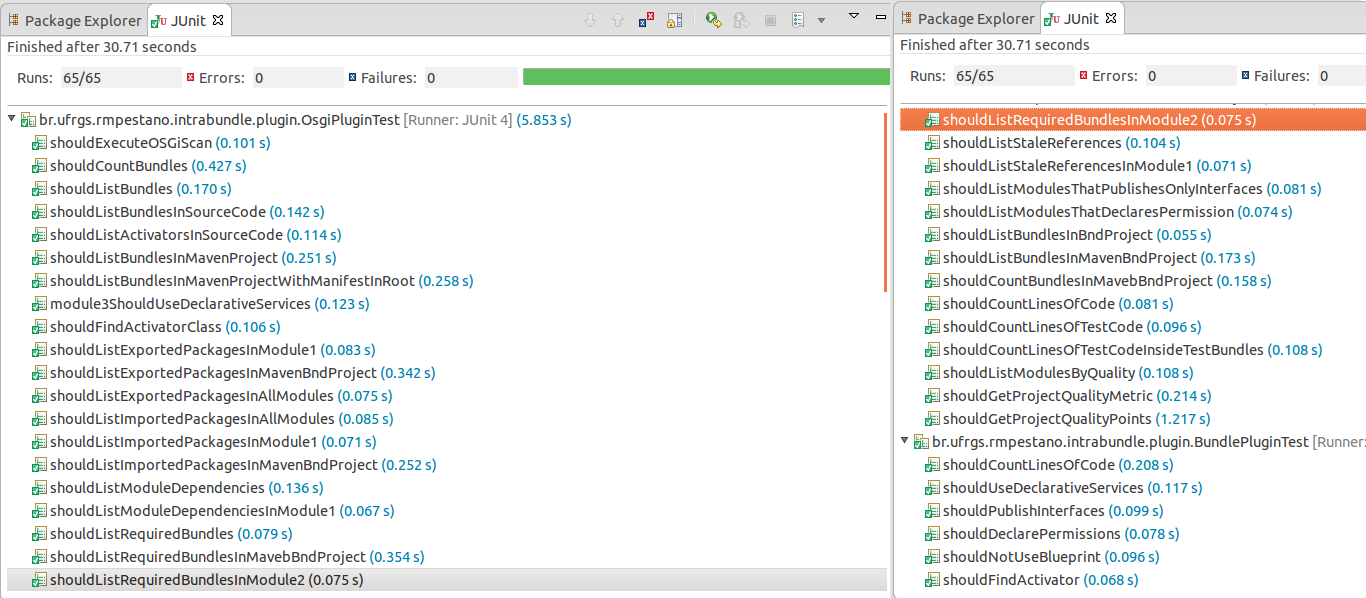
\includegraphics[scale=0.5]{intrabundle-external-quality}
\end{figure}

\FloatBarrier